\title{[Lab5] Conditional Sequence-to-Sequence VAE}
\author{0616014 楊政道}
\maketitle
\thispagestyle{fancy}
\section{Introduction}
\subsection{實驗目的}
\paragraph{}
本次實驗目的為用LAB4的seq2seq rnn model來建構一個conditional seq2seq VAE來完成英文單字的時態轉換以及用Gaussian Noise來生成出單字的4個時態。
\subsection{Dataset}
\paragraph{}
在訓練集中, 有1227種單字, 每種單字都有對應的4個時態變化, 例如(dart darts darting darted)分別對應到簡單式, 三單, 進行式還有過去式。 
\paragraph{}
而在測試資料集中, 有10個單字組, 每組單字組包含兩個同種單字但是不同時態, 用來測試CVAE的單字時態轉換能力。
\subsection{Project Structure}
\dirtree{%
.1 DLP\_LAB4\_0616014\_楊政道.zip.
.2 dataset/.
.3 dataloader.py.
.2 model/.
.3 Encoder.py.
.3 Decoder.py.
.3 Seq2Seq.py.
.2 weight/.
.3 record.json.
.2 train.py.
.2 evaluate.py.
}
\subsubsection{data/dataloader.py}
\paragraph{}
對train.txt和test.txt做資料處理, 並建構字母集來encode和decode字串和張量。
\subsubsection{model/Encoder.py}
\paragraph{}
定義Seq2Seq架構中Encoder的內容, 使用LSTM來實作。
\subsubsection{model/Decoder.py}
\paragraph{}
定義Seq2Seq架構中Decoder的內容, 使用LSTM來實作。
\subsubsection{model/Seq2Seq.py}
\paragraph{}
融合Encoder和Decoder兩個model, 並且加入了latent2hidden, mean-fc和logvar-fc這些結構, 來組合出完整的CVAE架構。
\subsubsection{weight/record.json}
\paragraph{}
若訓練出來的model在BLEU-4 score的表現上比之前的model weight還突出, 就紀錄起來。
\subsubsection{train.py}
\paragraph{}
定義train函數來訓練model。
\subsubsection{evaluate.py}
\paragraph{}
定義evalute函數來做時態轉換和Gaussian score測驗。
\section{Derivation of CVAE}
\paragraph{}
The marginal likelihoods of $x^{(i)}$
\begin{equation}
\begin{aligned}
log p_\theta(x^{(i)})
&= log p_\theta(x^{(i)}, z) - log p_\theta(z|x^{(i)}) \\
&= D_{KL}(q_\phi(z|x^{(i)})\|p_\theta(z|x^{(i)})) + L(\theta,\phi;x^{(i)}) \\
&\geq L(\theta, \phi;x^{(i)}) = E_{q_\phi(z|x^{(i)})}[-log q_\phi(z|x^{(i)})+log p_\theta(x^{(i)}, z)]
\end{aligned}
\end{equation}

\begin{equation}
\begin{aligned}
L(\theta, \phi;x^{(i)}) 
&= E_{q_\phi(z|x^{(i)})}[-log q_\phi(z|x^{(i)}) + log p_\theta(x^{(i)}|z)+log p_\theta(z)] \\
&= -D_{KL}(q_\phi(z|x^{(i)})\|p_\theta(z))+E_{q_\phi(z|x^{(i)})}[log p_\theta(x^{(i)}|z)]
\end{aligned}
\end{equation}
\section{Implementation details}
\subsection{DataLoader}
\subsubsection{Dictionary}
\paragraph{}
建立字母集, 其中包含encode和decode的操作方便轉換資料格式。
\begin{lstlisting}[language=Python]
class Dictionary:
    def __init__(self, sigma):
        self.char2idx = {'SOS': 0, 'EOS': 1, 'UNK': 2}
        self.idx2char = {0: '', 1: '', 2: '?'}

        for c in sigma:
            if c in self.char2idx:
                continue
            idx = len(self.char2idx)
            self.char2idx[c] = idx
            self.idx2char[idx] = c
    def encode(self, w):
        return torch.tensor(
              [ self.char2idx[c] if c in self.char2idx else 2 for c in w ]
            + [ 1 ],
        device=device).view(-1, 1)
    def decode(self, t):
        return ''.join([self.idx2char[v.item()] for v in t.view(-1)])
\end{lstlisting}
\subsubsection{TrainDataset}
\paragraph{}
訓練用資料讀出所有資料並且壓成一個維度, 可以用index來判斷該單字的時態。\_\_getitem\_\_則回傳該index的英文單字和時態。
\begin{lstlisting}[language=Python]
class TrainDataset(Dataset):
    def __init__(self, path):
        self.data = np.loadtxt(path, dtype=np.str).reshape(-1)
        self.dict = Dictionary("abcdefghijklmnopqrstuvwxyz")
        self.tense = {
            'sp': 0,
            'tp': 1,
            'pg': 2,
            'p': 3
        }
    def __len__(self):
        return len(self.data)
    def __getitem__(self, index):
        return self.data[index], index % len(self.tense)
\end{lstlisting}
\subsubsection{TestDataset}
\paragraph{}
測試用資料集為10組單字, 每組都是相同單字但是不同時態, 建立起每個pair對應的時態關係, 在\_\_getitem\_\_時把他們對應的單字和時態回傳。
\begin{lstlisting}[language=Python]
class TestDataset(Dataset):
    def __init__(self, path):
        self.data = np.loadtxt(path, dtype=np.str)
        self.dict = Dictionary("abcdefghijklmnopqrstuvwxyz")
        self.tense = {
            'sp': 0,
            'tp': 1,
            'pg': 2,
            'p': 3
        }
        self.target = [
            ['sp',  'p'],
            ['sp',  'pg'],
            ['sp',  'tp'],
            ['sp',  'tp'],
            ['p',   'tp'],
            ['sp',  'pg'],
            ['p',   'sp'],
            ['pg', 'sp'],
            ['pg', 'p'],
            ['pg', 'tp']
        ]
    def __len__(self):
        return len(self.data)
    def __getitem__(self, index):
        return self.data[index][0], self.tense[self.target[index][0]], self.data[index][1], self.tense[self.target[index][1]]
\end{lstlisting}
\subsection{Encoder}
\paragraph{}
Encoder要做的事情很單純, 就是將輸入的字母進去embedding function轉成一個向量, 然後在跟自己上一個hidden做LSTM運算即可。
\begin{lstlisting}[language=Python]
class EncoderRNN(nn.Module):
    def __init__(self, num_of_word, hidden_size):
        super(EncoderRNN, self).__init__()
        self.hidden_size = hidden_size
        self.embedding = nn.Embedding(num_of_word, hidden_size)
        self.lstm = nn.LSTM(hidden_size, hidden_size)
    def forward(self, input, hidden):
        embedded = self.embedding(input).view(input.size(0), 1, -1)
        output, hidden = self.lstm(embedded, hidden)
        return output, hidden
    def name(self):
        return f'EncoderRNN-{self.hidden_size}'
\end{lstlisting}
\subsection{Decoder}
\paragraph{}
Decoder要做的事情也很單純, 也是將輸入的字母進去embedding function轉成向量, 再和自己上一個hidden做LSTM運算, output再接一個fc來預測這次要輸出的字母是什麼。
\begin{lstlisting}[language=Python]
class DecoderRNN(nn.Module):
    def __init__(self, num_of_word, hidden_size):
        super(DecoderRNN, self).__init__()
        self.hidden_size = hidden_size
        self.embedding = nn.Embedding(num_of_word, hidden_size)
        self.lstm = nn.LSTM(hidden_size, hidden_size)
        self.out = nn.Linear(hidden_size, num_of_word)
    def forward(self, input, hidden):
        output = self.embedding(input).view(1, 1, -1)
        output = F.relu(output)
        output, hidden = self.lstm(output, hidden)
        output = self.out(output[0])
        return output, hidden
    def name(self):
        return f'DecoderRNN-{self.hidden_size}'
\end{lstlisting}
\subsection{CVAE}
\paragraph{}
CVAE在training的階段時, 會收到一個單字和他的時態, 目標是要讓encoder學到資料的分佈, 並讓該分佈趨近於N(0, 1), 再讓decoder成功解出該單字。其中encoder的初始hidden要塞入conditional vector, 可以從condition\_embedding\_function得出。
\paragraph{}
離開encoder時, 要將encoder的hidden經過兩個fc, 一個代表該分佈的平均值, 另一個代表該分佈的log變異數。
\paragraph{}
要進到decoder前, 要將估測出的平均值和log變異數平移縮放N(0, 1)並接上conditional vector, 形成decoder的新hidden,再讓decoder生出對應的單字。
\begin{lstlisting}[language=Python]
class Seq2Seq(nn.Module):
    def __init__(self, hidden_size, num_of_word, cond_size, num_of_cond, latent_size):
        super(Seq2Seq, self).__init__()
        self.cond_embedding = nn.Embedding(num_of_cond, cond_size)
        self.encoder = EncoderRNN(num_of_word, hidden_size)
        self.mean = nn.Linear(hidden_size, latent_size)
        self.logvar = nn.Linear(hidden_size, latent_size)
        self.latent2hidden = nn.Linear(latent_size + cond_size, hidden_size)
        self.latent2cell = nn.Linear(latent_size + cond_size, hidden_size)
        self.decoder = DecoderRNN(num_of_word, hidden_size)
        self.hidden_size = hidden_size
        self.cond_size = cond_size
        self.latent_size = latent_size
    def condition(self, c):
        return self.cond_embedding(torch.LongTensor([c]).to(device)).view(1, 1, -1)
    def sample_z(self):
        return torch.normal(
            torch.FloatTensor([0] * (self.latent_size)),
            torch.FloatTensor([1] * (self.latent_size))
        ).to(device).view(1, 1, -1)
    def initHidden(self, hidden, cell, cond):
        return (
            torch.cat((hidden, cond), dim=2),
            cell
        )
    def forward(self, input, input_c, target, target_c, use_teacher_forcing):
        output, hidden = self.encoder(
            input,
            self.initHidden(
                torch.zeros(self.hidden_size - self.cond_size, device=device).view(1, 1, -1),
                torch.zeros(self.hidden_size, device=device).view(1, 1, -1),
                self.condition(input_c)
            )
        )
        m = self.mean(hidden[0])
        lgv = self.logvar(hidden[0])
        z = self.sample_z() * torch.exp(lgv / 2) + m
        hidden = (
            self.latent2hidden(torch.cat((z, self.condition(target_c)), dim=2).reshape(-1)).view(1, 1, -1),
            self.latent2cell(torch.cat((z, self.condition(target_c)), dim=2).reshape(-1)).view(1, 1, -1)
        )
        input = torch.tensor([[0]], device=device)
        ret = []
        for i in range(MAX_LENGTH):
            output, hidden = self.decoder(input, hidden)
            if use_teacher_forcing:
                if i == target.size(0):
                    break
                ret.append(output)
                input = target[i]
            else:
                ret.append(output)
                topv, topi = output.topk(1)
                input = topi.squeeze().detach()
                if input.item() == 1:
                    break
        return torch.stack(ret), m, lgv
\end{lstlisting}
\paragraph{}
生成文字的機率分佈使用sample\_z(), 他是一個Gaussian noise
\begin{lstlisting}[language=Python]
    def sample_z(self):
        return torch.normal(
            torch.FloatTensor([0] * (self.latent_size)),
            torch.FloatTensor([1] * (self.latent_size))
        ).to(device).view(1, 1, -1)
\end{lstlisting}
\subsection{Hyperparameters}
\begin{itemize}
\item KL weight: monotonic and cyclical
\item learning rate: 0.5
\item teacher forcing ratio: 0.6
\end{itemize}
\newpage
\section{Results and discussion}
\paragraph{}
訓練時可以觀察CrossEntropyLoss和KLLoss來評斷該CVAE的學習狀況, 如果CrossEntropyLoss愈小, 時態轉換上和生成單字的正確性就會來得比較好, 但是在使用Gaussian Noise來生成單字的表現就會比較差, 原因是Decoder所希望接收的資料分佈當KLLoss很大時並不是Gaussian Noise, 所以表現就會變差。相反的, 如果KLLoss降低, 可以讓Decoder接收到的資料分佈愈靠近Gaussian Noise分佈, 因次在generation的表現上就會有所提升, 但是CrossEntropy上升會導致時態轉換和單字正確性下降。所以訓練的目標就是如何讓兩個Loss下降, 仰賴於調整KLD\_weight。
\paragraph{}
若KLD\_weight設定過大, 會讓Loss function較偏向於KLLoss而倒置VAE無法輸出正確且精準的英文單字還有時態轉換。相反的, 若KLD\_weight設定過小, 雖然在英文單字時態轉換的BLEU分數很高, 但是由於資料分佈並不是趨近於N(0, 1), 在generation時表現就會很差。
\subsection{Plot during Training}
\subsubsection{Monotonic}
\begin{figure}[!ht]
    \begin{center} 
        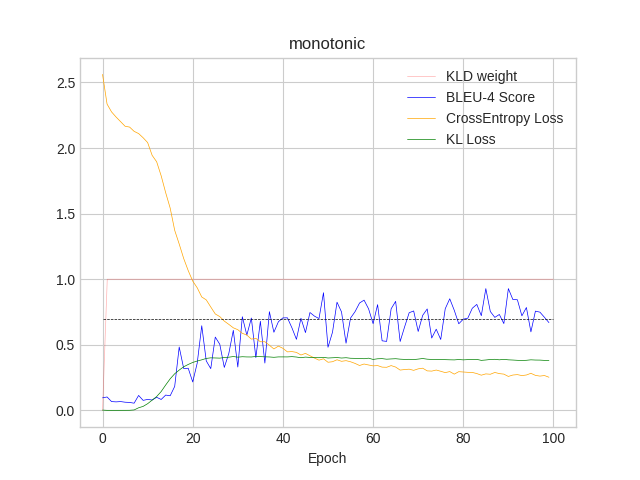
\includegraphics[width=8cm]{monotonic.png}
        \caption{Monotonic KLD weight}
    \end{center} 
\end{figure}
\subsubsection{Cyclical}
\begin{figure}[!ht]
    \begin{center} 
        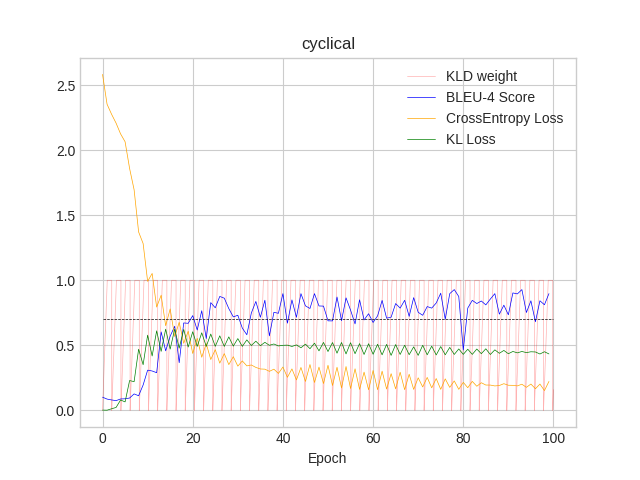
\includegraphics[width=8cm]{cyclical.png}
        \caption{Cyclical KLD weight}
    \end{center} 
\end{figure}
\paragraph{}
可以看出兩個不同的annealing策略,結果有些許不同。
\paragraph{}
第1種是Monotonic的方法來調整KLD\_weight, 前期先讓CrossEntropyLoss訓練下來, 讓VAE的輸出先稍微穩定再來調整資料的分佈, 但這就很吃調整前期KLD\_weight的爬升速度, 如果爬得太快會讓CrossEntropyLoss來不及訓練好就受到KLLoss的影響, 而使得訓練的結果不理想或是收斂速度太慢。
\paragraph{}
第2種是Cyclical的策略, 此種方法讓CrossEntropyLoss和KLLoss輪流下降, 可以從圖中看到當KLD\_weight上升的時候, 因為在Loss function KLLoss的比重增加, 而CrossEntropyLoss就會上升, KLLoss就會下降。相反的, 當KLD\_weight掉回0的時候, 就是CrossEntropyLoss下降的時機, 但是會使得KLLoss上升。經過多次的循環, CrossEntropyLoss和KLLoss都會慢慢下降。
\paragraph{}
從這兩張圖可以看出, Cyclical策略的前期收斂速度會比Monotonic來得快, 後期的在CrossEntropyLoss的表現也比較優異。
\subsection{Tense conversion}
\begin{lstlisting}
< abandon
= abandoned
> abandoned
----------------------
< abet
= abetting
> abetting
----------------------
< begin
= begins
> begins
----------------------
< expend
= expends
> expends
----------------------
< sent
= sends
> sends
----------------------
< split
= splitting
> splitting
----------------------
< flared
= flare
> flare
----------------------
< functioning
= function
> function
----------------------
< functioning
= functioned
> functioned
----------------------
< healing
= heals
> heals
----------------------
BLEU-4 score: 1.0
\end{lstlisting}
\paragraph{}
可以看到CVAE可以完成英文單字的時態轉換。
\subsection{Generation}
\begin{lstlisting}
     blimm          	blimme         	blimming       	blimmed        	
     bestae         	bestains       	bestaining     	bestaeee       	
---> ensue          	ensues         	ensuing        	ensued         	
     specion        	specceee       	specceeing     	spinsered      	
     undrruc        	undrruses      	undrruiing     	undrruted      	
---> achieve        	achieves       	achieving      	achieved       	
     tett           	tetts          	tetting        	tetted         	
---> recover        	recovers       	recovering     	recovered      	
---> stalk          	stalks         	stalking       	stalked        	
     bronn          	bronns         	bronning       	bronned        	
---> stalk          	stalks         	stalking       	stalked        	
---> abet           	abets          	abetting       	abetted        	
     seet           	seets          	seeting        	set            	
---> chance         	chances        	chancing       	chanced        	
---> confess        	confesses      	confessing     	confessed      	
---> crush          	crushes        	crushing       	crushed        	
---> apprise        	apprises       	apprising      	apprised       	
     overflae       	overflaes      	overflaiin     	overflaed      	
     charge         	charges        	charging       	chargeeed      	
     baught         	bausts         	bausting       	baught         	
     essape         	escapes        	escapinng      	escaped        	
     blust          	blushes        	blushing       	blusted        	
---> breach         	breaches       	breaching      	breached       	
     wid            	wids           	widing         	wided          	
     consent        	consents       	consening      	consented      	
     boll           	bolls          	bolling        	bolled         	
     cartwhre       	cartwhrs       	cartwhriing    	cartwhre       	
---> kill           	kills          	killing        	killed         	
     twish          	twishes        	twishing       	twished        	
     breater        	berrares       	berearing      	berrared       	
     prohibit       	inslifies      	prohibiting    	prohibieed     	
---> dip            	dips           	dipping        	dipped         	
---> devise         	devises        	devising       	devised        	
---> supplement     	supplements    	supplementing  	supplemented   	
---> drag           	drags          	dragging       	dragged        	
---> display        	displays       	displaying     	displayed      	
     corre          	coreeds        	coreeing       	coarned        	
     dismiss        	disagies       	disagreing     	disagiee       	
     decline        	declines       	decliniing     	declined       	
     coillot        	coillots       	coilicing      	coiliced       	
---> grope          	gropes         	groping        	groped         	
     smoth          	smotts         	shutting       	shutted        	
     flap           	flaps          	flaping        	flaped         	
---> switch         	switches       	switching      	switched       	
---> resound        	resounds       	resounding     	resounded      	
     conmemn        	commands       	conmending     	commanded      	
     dive           	dives          	diving         	dived          	
     negglf         	blistsss       	blistting      	blistted       	
     saitocize      	switicaee      	switictiig     	switicted      	
---> preserve       	preserves      	preserving     	preserved      	
---> arrange        	arranges       	arranging      	arranged       	
---> resign         	resigns        	resigning      	resigned       	
---> stimulate      	stimulates     	stimulating    	stimulated     	
---> flail          	flails         	flailing       	flailed        	
     befit          	beits          	befiting       	befit          	
     fill           	fixes          	fixing         	fixed          	
     exerr          	exerrs         	exerring       	exerred        	
     attract        	attaches       	attaching      	attached       	
     foreach        	foreaches      	foreaching     	foreached      	
     nuffer         	nuffers        	nuffering      	nuffered       	
     feel           	feels          	feeling        	feel           	
     pay            	pays           	paying         	had            	
---> exhibit        	exhibits       	exhibiting     	exhibited      	
     disagree       	disagrees      	disagreing     	disagreed      	
---> strut          	struts         	strutting      	strutted       	
     surrod         	murmurs        	murmuring      	murmured       	
     decogniee      	decognies      	decoensing     	decoonaedd     	
     permi          	permies        	permiing       	permied        	
     divd           	divds          	dividing       	divded         	
     cxptcipate     	disqualifies   	cxptcipating   	disqualified   	
---> feign          	feigns         	feigning       	feigned        	
---> whack          	whacks         	whacking       	whacked        	
     oversle        	respects       	oepleping      	oepleped       	
---> abuse          	abuses         	abusing        	abused         	
     contine        	contines       	contining      	contined       	
---> disobey        	disobeys       	disobeying     	disobeyed      	
---> delay          	delays         	delaying       	delayed        	
     trotibute      	trotibutes     	trotibuting    	trotibuted     	
---> approve        	approves       	approving      	approved       	
     covvice        	composes       	covvicing      	composed       	
---> persist        	persists       	persisting     	persisted      	
---> wax            	waxes          	waxing         	waxed          	
     concern        	concerns       	concerning     	accourted      	
---> delude         	deludes        	deluding       	deluded        	
     leet           	meets          	leeting        	leet           	
---> poison         	poisons        	poisoning      	poisoned       	
---> continue       	continues      	continuing     	continued      	
     sesturt        	sesturts       	sesturting     	smothered      	
     deam           	deams          	deaming        	deamed         	
     congaaae       	cirgulates     	congaaiing     	congaaled      	
     chance         	chances        	chancing       	crenched       	
     precede        	preeeee        	preceding      	preeeedd       	
     eoss           	eosss          	eossing        	eossed         	
     accipt         	accipts        	accipting      	accipted       	
     absign         	absirbs        	absigning      	absirbed       	
     bleck          	blecks         	blecking       	blecked        	
     jab            	jabs           	jabing         	jabed          	
     express        	express        	expresing      	expresed       	
     receive        	records        	reterring      	reterred       	
     oummon         	oumpans        	obcaiding      	obtained       	
Gaussian score: 0.42
\end{lstlisting}
\paragraph{}
在generation的表現上, CVAE也有超過4成的資料是出現在訓練資料內的。(--->標示的為在訓練資料內的單字)
